\documentclass{standalone}

\usepackage[utf8] {inputenc}
\usepackage[T2A]{fontenc}
\usepackage[english, russian] {babel}
\usepackage[usenames,dvipsnames]{xcolor}
\usepackage{graphics}

\usepackage{pscyr}
\renewcommand{\rmdefault}{ftm}
\begin{document}
% Title: gl2ps_renderer figure
% Creator: GL2PS 1.4.0, (C) 1999-2017 C. Geuzaine
% For: Octave
% CreationDate: Mon May 14 16:50:55 2018
\setlength{\unitlength}{1pt}
\begin{picture}(0,0)
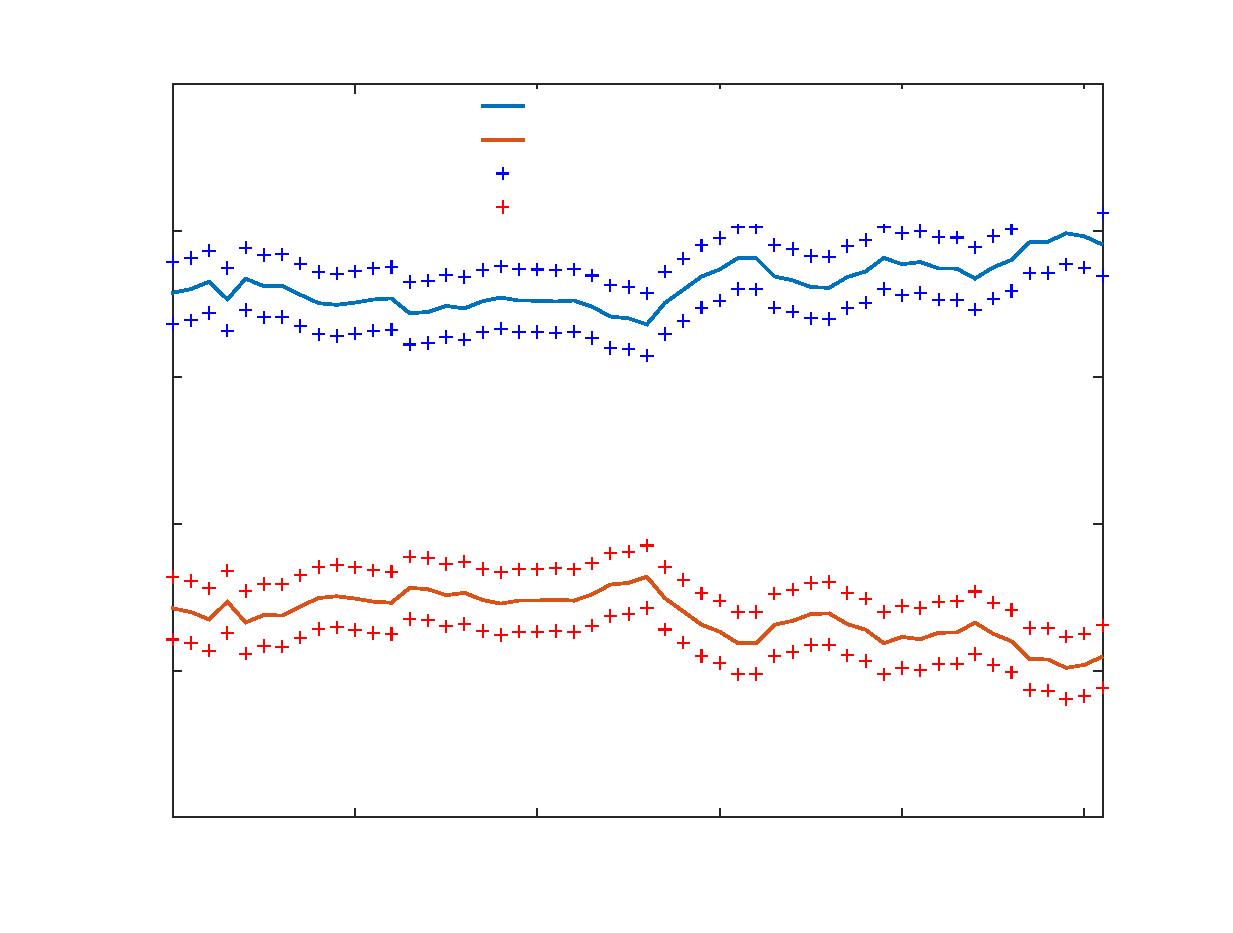
\includegraphics{p-inc}
\end{picture}%
\begin{picture}(576,432)(0,0)
\fontsize{10}{0}
\selectfont\put(74.88,42.5189){\makebox(0,0)[t]{\textcolor[rgb]{0.15,0.15,0.15}{{30}}}}
\fontsize{10}{0}
\selectfont\put(162.409,42.5189){\makebox(0,0)[t]{\textcolor[rgb]{0.15,0.15,0.15}{{40}}}}
\fontsize{10}{0}
\selectfont\put(249.939,42.5189){\makebox(0,0)[t]{\textcolor[rgb]{0.15,0.15,0.15}{{50}}}}
\fontsize{10}{0}
\selectfont\put(337.468,42.5189){\makebox(0,0)[t]{\textcolor[rgb]{0.15,0.15,0.15}{{60}}}}
\fontsize{10}{0}
\selectfont\put(424.998,42.5189){\makebox(0,0)[t]{\textcolor[rgb]{0.15,0.15,0.15}{{70}}}}
\fontsize{10}{0}
\selectfont\put(512.527,42.5189){\makebox(0,0)[t]{\textcolor[rgb]{0.15,0.15,0.15}{{80}}}}
\fontsize{10}{0}
\selectfont\put(69.8755,47.52){\makebox(0,0)[r]{\textcolor[rgb]{0.15,0.15,0.15}{{0}}}}
\fontsize{10}{0}
\selectfont\put(69.8755,117.936){\makebox(0,0)[r]{\textcolor[rgb]{0.15,0.15,0.15}{{0.2}}}}
\fontsize{10}{0}
\selectfont\put(69.8755,188.352){\makebox(0,0)[r]{\textcolor[rgb]{0.15,0.15,0.15}{{0.4}}}}
\fontsize{10}{0}
\selectfont\put(69.8755,258.768){\makebox(0,0)[r]{\textcolor[rgb]{0.15,0.15,0.15}{{0.6}}}}
\fontsize{10}{0}
\selectfont\put(69.8755,329.184){\makebox(0,0)[r]{\textcolor[rgb]{0.15,0.15,0.15}{{0.8}}}}
\fontsize{10}{0}
\selectfont\put(69.8755,399.6){\makebox(0,0)[r]{\textcolor[rgb]{0.15,0.15,0.15}{{1}}}}
\fontsize{15}{0}
\selectfont\put(298.08,29.5188){\makebox(0,0)[t]{\textcolor[rgb]{0.15,0.15,0.15}{{Время, s}}}}
\fontsize{15}{0}
\selectfont\put(50.8755,223.56){\rotatebox{90}{\makebox(0,0)[b]{\textcolor[rgb]{0.15,0.15,0.15}{{Процент ПС}}}}}
\fontsize{10}{0}
\selectfont\put(246.303,388.796){\makebox(0,0)[l]{\textcolor[rgb]{0,0,0}{{Процент ПС для класса 2}}}}
\fontsize{10}{0}
\selectfont\put(246.303,372.678){\makebox(0,0)[l]{\textcolor[rgb]{0,0,0}{{Процент ПС для класса 1}}}}
\fontsize{10}{0}
\selectfont\put(246.303,356.561){\makebox(0,0)[l]{\textcolor[rgb]{0,0,0}{{Доверительный интервал для значений класса 2}}}}
\fontsize{10}{0}
\selectfont\put(246.303,340.444){\makebox(0,0)[l]{\textcolor[rgb]{0,0,0}{{Доверительный интервал для значений класса 1}}}}
\end{picture}
\end{document}
